\begin{name}
{Đề Ôn Tập HS TB-Yếu}
{Năm học 2025-2026}
\end{name}

\Opensolutionfile{ans}[ans/De-TB-Yeu-So-6]
\cautn
\begin{ex}%[1D2N2-2]
	Trong các dãy số sau, dãy nào là cấp số cộng?
	\choice
	{$\dfrac{1}{2}$; $\dfrac{2}{3}$; $1$; $\dfrac{4}{3}$; $2$}
	{\True $5$; $2$; $-1$; $-4$; $-7$}
	{$1$; $4$; $7$; $10$; $14$}
	{$-3$; $1$; $5$; $9$; $14$}
	\loigiai{
		$5$; $2$; $-1$; $-4$; $-7$ là cấp số cộng vì $2-5=-1-2=-4-(-1)=-7-(-4)=-3$.
	}
\end{ex}

\begin{ex}%[2H5N1-5]
	Trong không gian $Oxyz$, khoảng cách của điểm $M(1,2,3)$ đến mặt $(Oxy)$ là
	\choice
	{$\sqrt{14}$}
	{$1$}
	{$2$}
	{\True $3$}
	\loigiai{
		Ta có $\mathrm{d}(M,(Oxy))=|z_M|=|3|=3$.
	}
\end{ex}

\begin{ex}%[1H8N7-3]
	Cho hình chóp $S.ABCD$ có đáy $ABCD$ là hình vuông cạnh $a$, cạnh bên $SA$ vuông góc với mặt phẳng đáy và $SA=a\sqrt{2}$. Thể tích của khối chóp đã cho bằng
	\choice
	{\True $\dfrac{a^3\sqrt{2}}{3}$}
	{$a^3\sqrt{2}$}
	{$\dfrac{a^3\sqrt{2}}{6}$}
	{$\dfrac{a^3\sqrt{2}}{4}$}
	\loigiai{
		Diện tích đáy $S_{ABCD}=a^2$.\\
		Thể tích của khối chóp đã cho là $V_{S.ABCD}=\dfrac{1}{3}SA\cdot S_{ABCD}=\dfrac{1}{3}a\sqrt{2}\cdot a^2=\dfrac{a^3\sqrt{2}}{3}$.
	}
\end{ex}

\begin{ex}%[1D5N1-2]
	Tổng hợp kết quả $30$ lần quả ném của bạn Văn, ta được bảng tần số ghép nhóm theo mẫu sau
	\begin{longtable}{|l|c|c|c|c|c|}
		\hline
		Cự li ($m$) & $[69{,}2;70)$ & $[70;70{,}8)$ & $[70{,}8;71{,}6)$ & $[71{,}6;72{,}4)$ & $[72{,}4;73{,}2)$ \\
		\hline
		Số lần & $7$ & $8$ & $5$ & $4$ & $6$ \\
		\hline
	\end{longtable}
	Số đại diện của nhóm $[70;70{,}8)$ là
	\choice
	{\True $70{,}4$}
	{$0{,}8$}
	{$70{,}8$}
	{$70$}
	\loigiai{
		Ta có $\dfrac{u_{j+1}+u_j}{2}=\dfrac{70+70{,}8}{2}=70{,}4$.
	}
\end{ex}

\begin{ex}%[1D6N2-1]
	Với $a$, $b$ là các số thực dương, $a\ne1$. Biểu thức $\log _a\left(a^2b\right)$ bằng
	\choice
	{\True $2+\log _ab$}
	{$1+2\log _ab$}
	{$2\log _ab$}
	{$2-\log _ab$}
	\loigiai{
		Ta có $\log _a\left(a^2b\right)=\log _aa^2+\log _ab=2\log _aa+\log _ab=2+\log _ab$.
	}
\end{ex}

\begin{ex}%[1H8N6-1]
	Cho hình chóp $S.ABC$ có $SA\perp (ABC)$. Góc giữa $SA$ và $(ABC)$ bằng
	\choice
	{$60^\circ$}
	{\True $90^\circ$}
	{$45^\circ$}
	{$30^\circ$}
	\loigiai{
		Do $SA\perp (ABC)$ nên góc giữa $SA$ và $(ABC)$ bằng $90^\circ$.
	}
\end{ex}

\begin{ex}%[2D1N4-1]
	Cho hàm số $y=f(x)$ có bảng biến thiên như hình vẽ sau
	\begin{center}
		
\begin{tikzpicture}
			\tkzTabInit[nocadre=false,lgt=1,espcl=2.5]{$x$ /0.6,$y'$ /0.6,$y$ /2.5}{$-\infty$,$0$,$1$,$+\infty$}
			\tkzTabLine{,-,d,+,0,-,}
			\tkzTabVar{+/ $+\infty$, -D-/ $-1$ / $-\infty$, +/ $2$, -/ $-\infty$}
		\end{tikzpicture}
	\end{center}
	Tổng số đường tiệm cận đứng và ngang của đồ thị hàm số $y=f(x)$ là
	\choice
	{\True $1$}
	{$3$}
	{$2$}
	{$0$}
	\loigiai{
		Ta có
		$\lim \limits_{x\to 0^+}y=-\infty\Rightarrow x=0$ là đường tiệm cận đứng. \\
		$\lim \limits_{x\to -\infty}y=-\infty$; $\lim \limits_{x\to +\infty}y=-\infty\Rightarrow$ nên đồ thị hàm số không có đường tiệm cận ngang.
	}
\end{ex}

\begin{ex}%[2D4N1-4]
	Hàm số $F(x)=x+\dfrac{1}{x}$ là một nguyên hàm của hàm số nào sau đây?
	\choice
	{$f(x)=1-\ln |x|$}
	{\True $f(x)=1-\dfrac{1}{x^2}$}
	{$f(x)=\dfrac{x^2}{2}-\ln |x|+C$}
	{$f(x)=\dfrac{x^2}{2}-\dfrac{1}{x^2}$}
	\loigiai{
		Ta có $f(x)=F'(x)=1-\dfrac{1}{x^2}$.
	}
\end{ex}

\begin{ex}%[2D1H2-1]
	Cho hàm số $y=f(x)$ xác định trên $\mathbb{R}$ và có bảng xét dấu của đạo hàm như sau
	\begin{center}
		
\begin{tikzpicture}
			\tkzTabInit[nocadre=false,lgt=1,espcl=2.5]{$x$ /0.6,$y'$ /0.6}{$-\infty$,$x_1$,$x_2$,$x_3$,$+\infty$}
			\tkzTabLine{,-,0,+,d,-,0,+,}
		\end{tikzpicture}
	\end{center}
	Khi đó số điểm cực trị của hàm số $y=f(x)$ là
	\choice
	{\True $3$}
	{$1$}
	{$4$}
	{$2$}
	\loigiai{
		Do hàm số $y=f(x)$ xác định trên $\mathbb{R}$ nên có bảng biến thiên
		\begin{center}
			
\begin{tikzpicture}
				\tkzTabInit[nocadre=false,lgt=1.2,espcl=2]{$x$ /1,$y'$ /1,$y$ /2}{$-\infty$,$x_1$,$x_2$,$x_3$,$+\infty$}
				\tkzTabLine{,-,0,+,d,-,0,+,}
				\tkzTabVar{+/ , -/ $f(x_1)$, +/ $f(x_2)$, -/ $f(x_3)$, +/ }
			\end{tikzpicture}
		\end{center}
		Vậy số đã cho có $3$ điểm cực trị.
	}
\end{ex}

\begin{ex}%[1D9N1-3]
	Cho hai biến cố độc lập $A,B$ với $\mathrm{P}(A)=0{,}6$, $\mathrm{P}(B)=0{,}45$. Khi đó, $\mathrm{P}(B\mid A)$ bằng
	\choice
	{$0{,}15$}
	{$0{,}75$}
	{$0{,}6$}
	{\True $0{,}45$}
	\loigiai{
		Vì $A$, $B$ là hai biến cố độc lập nên $\mathrm{P}(B)=\mathrm{P}(B\mid A)=0{,}45$.
	}
\end{ex}

\begin{ex}%[2H5H3-3]
	Trong không gian với hệ tọa độ $Oxyz$ cho tam giác $ABC$ có $A(2;2;0)$, $B(1;0;2)$, $C(0;4;4)$. Viết phương trình mặt cầu có tâm là $A$ và đi qua trọng tâm $G$ của tam giác $ABC$.
	\choice
	{$(x-2)^2+(y-2)^2+z^2=4$}
	{$(x-2)^2+(y-2)^2+z^2=\sqrt{5}$}
	{$(x+2)^2+(y+2)^2+z^2=5$}
	{\True $(x-2)^2+(y-2)^2+z^2=5$}
	\loigiai{
		Gọi $G$ là trọng tâm tam giác $ABC$ khi đó ta có $G(1;2;2)\Rightarrow \overrightarrow{AG}=(-1;0;2)\Rightarrow \left|\overrightarrow{AG}\right|=\sqrt{5}$. \\
		Phương trình mặt cầu tâm $A$ và đi qua trọng tâm $G$ của tam giác $ABC$ là
		$$(x-2)^2+(y-2)^2+z^2=5.$$
	}
\end{ex}

\begin{ex}%[1D6N4-2]
	Nghiệm của phương trình $2^x=4$ là
	\choice
	{\True $x=2$}
	{$x=-3$}
	{$x=-2$}
	{$x=3$}
	\loigiai{
		Ta có $2^x=4\Leftrightarrow x=2$.
	}
\end{ex}

\cauds
\begin{ex}%[2D5H1-2]
	Một hộp có $10$ bi xanh và $8$ bi đen, các viên bi đều có cùng hình dáng, kích thước và khối lượng. Bạn Nam lấy ngẫu nhiên một viên trong hộp, không trả lại. Sau đó Bạn Lan lấy ngẫu nhiên một trong $17$ viên bi còn lại. Gọi $A$ là biến cố bạn Nam lấy được một viên bi xanh và $B$ là biến cố bạn Lan lấy được một viên bi đen.
	\choiceTF
	{\True $\mathrm{P}\left(A\right)=\dfrac{5}{9}$}
	{$\mathrm{P}\left(AB\right)=0{,}8$}
	{\True $n(A)=10$}
	{$\mathrm{P}\left(B\mid A\right)=\dfrac{4}{9}$}
	\loigiai{
		\begin{itemchoice}
			\itemch Vì bạn Nam lấy ngẫu nhiên $1$ viên bi từ hộp chứa $10$ bi xanh và $8$ bi đen nên $n(\Omega )=18$.\\
			Số phần tử của biến cố $A$ là $n(A)=10$.\\
			Do đó, $\mathrm{P}\left(A\right)=\dfrac{n(A)}{n(\Omega )}=\dfrac{10}{18}=\dfrac{5}{9}$.
			\itemch Áp dụng công thức nhân xác suất, ta có $\mathrm{P}\left(AB\right)=\mathrm{P}\left(A\right)\cdot \mathrm{P}\left(B\mid A\right)=\dfrac{5}{9}\cdot \dfrac{8}{17}=\dfrac{40}{153}\approx0{,}3$.
			\itemch Vì hộp có $10$ bi xanh nên số phần tử của biến cố $A$ là $n(A)=10$.
			\itemch Nếu $A$ xảy ra tức là bạn Nam lấy được bi xanh thì trong hộp còn lại $17$ viên bi với $8$ bi đen.\\
			Do đó, $\mathrm{P}\left(B\mid A\right)=\dfrac{8}{17}$.
		\end{itemchoice}
	}
\end{ex}

\begin{ex}%[2D4V3-2]
	\immini[thm]
	{Một người nông dân có một mảnh đất hình vuông $ABCD$ cạnh bằng $8$ m. Ông ta định chia mảnh đất thành ba phần, bởi các parabol đi qua các đỉnh của hình vuông như hình vẽ, biết rằng đỉnh của parabol cách cạnh hình vuông $2$ m. Ông dự định trồng hoa trên phần diện tích giới hạn bởi các parabol và cạnh hình vuông, trồng cỏ trên phần diện tích còn lại.
		Chọn hệ trục $Oxy$ sao cho $A(-4;4)$, $B(4;4)$, $C(4;-4)$, $D(-4;-4)$.}
	{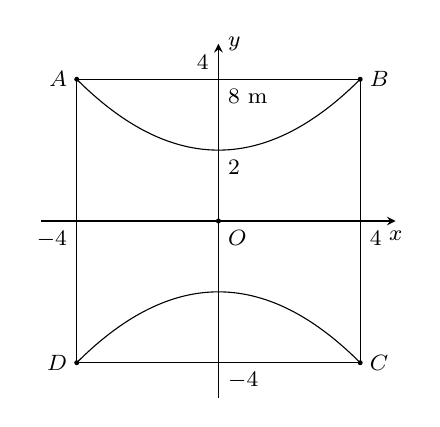
\begin{tikzpicture}[scale=0.45, >=stealth, font=\footnotesize]
			\draw[->] (-5,0) -- (5,0) node[below] {$x$};
			\draw[->] (0,-5) -- (0,5) node[right] {$y$};
			\node[below right] at (0,0) {$O$};
			
			\draw (-4,4) -- (4,4) node[midway, below right] {$8$ m} -- (4,-4) -- (-4,-4) -- cycle;
			\draw[domain=-4:4, samples=100] plot (\x, {\x*\x/8 + 2});
			\draw[domain=-4:4, samples=100] plot (\x, {-\x*\x/8 - 2});
			
			\node[left] at (-4,4) {$A$};
			\node[right] at (4,4) {$B$};
			\node[right] at (4,-4) {$C$};
			\node[left] at (-4,-4) {$D$};
			
			\node[above left] at (0,4) {$4$};
			\node[below right] at (0,2) {$2$};
			\node[below right] at (0,-4) {$-4$};
			\node[below right] at (4,0) {$4$};
			\node[below left] at (-4,0) {$-4$};
			\foreach \point in {(-4,4), (4,4), (4,-4), (-4,-4), (0,0)} {
				\fill \point circle (2pt);
			}
	\end{tikzpicture}}
	\choiceTF
	{\True Phương trình của hai parabol là $y=\dfrac{x^2}{8}+2$ và $y=-\dfrac{x^2}{8}-2$}
	{\True Diện tích trồng hoa bằng $\dfrac{44}{3}$ m$^2$}
	{Nếu chi phí mua cây giống hoa là $100\,000$ đồng/m$^2$, cỏ là $70\,000$ đồng/m$^2$ thì chi phí mua cây giống cho cả khu vườn là $4\,900\,000$ đồng}
	{Tỉ số diện tích đất trồng hoa và trồng cỏ bằng $\dfrac{11}{37}$}
	\loigiai{
		\begin{itemchoice}
			\itemch Phương trình parabol có dạng $y=f(x)=ax^2+bx+c\ (P)$.\\
			Ta có $A(-4;4)$, $B(4;4)$, $E(0;2)\in (P)\Rightarrow y=\dfrac{x^2}{8}+2$.\\
			Tương tự, phương trình parabol thứ hai là $y=-\dfrac{x^2}{8}-2$.
			\itemch Gọi $S_1$ là diện tích hình phẳng giới hạn bởi parabol $y=\dfrac{x^2}{8}+2$, đường thẳng $y=4$ và hai đường thẳng $x=0$, $x=4$.\\
			Diện tích đất trồng hoa là $$S=4S_1=4\int \limits_0^4\left[4-\left(\dfrac{x^2}{8}+2\right)\right]\mathrm{\,d}x=4\left(-\dfrac{x^3}{24}+2x\right)\bigg|_0^4=\dfrac{44}{3}\text{ m}^2.$$
			\itemch Chi phí mua cây giống là $\dfrac{44}{3}\cdot 100\,000+\dfrac{148}{3}\cdot 70\,000=4\,920\,000$ đồng.
			\itemch Diện tích đất trồng cỏ là $S'=64-S=64-\dfrac{44}{3}=\dfrac{148}{3}\text{ m}^2$.\\
			Tỉ số diện tích đất trồng hoa và trồng cỏ là $\dfrac{S}{S'}=\dfrac{11}{37}$.
		\end{itemchoice}
	}
\end{ex}

\begin{ex}%[2D1H4-1]
	Cho hàm số $y=\dfrac{-x^2-3x+4}{x-3}$ có đồ thị $(C)$.
	\choiceTF
	{\True Đồ thị $(C)$ có hai điểm cực trị nằm $2$ phía đối với $Oy$}
	{\True Đồ thị $(C)$ nhận giao điểm $I(3;-9)$ làm tâm đối xứng}
	{Đồ thị không cắt trục $Ox$}
	{\True Đồ thị $(C)$ có tiệm cận xiên là $y=-x-6$}
	\loigiai{
		\begin{itemchoice}
			\itemch Ta có $y'=\dfrac{-x^2+6x+5}{(x-3)^2}=0\Leftrightarrow -x^2+6x+5=0$ $(*)$.\\
			Phương trình $(*)$ luôn có $2$ nghiệm $x_1<0<x_2$.\\
			Nên đồ thị luôn có $2$ điểm cực trị nằm $2$ phía đối với $Oy$.
			\itemch Ta có $y=-x-6-\dfrac{14}{x-3}$.\\
			Khi đó tiệm cận xiên là $y=-x-6$, tiệm cận đứng là $x=3$.\\
			Suy ra, giao điểm $2$ tiệm cận là $I(3;-9)$ là tâm đối xứng.
			\itemch Ta có  $y=0\Leftrightarrow -x^2-3x+4=0\Leftrightarrow \hoac{&x=1\\&x=-4.}$\\
			Phương trình luôn có $2$ nghiệm phân biệt. Suy ra đồ thị cắt trục $Ox$ tại hai điểm phân biệt.
			\itemch Ta có $y=\dfrac{-x^2-3x+4}{x-3}=-x-6-\dfrac{14}{x-3}$.\\
			Khi đó tiệm cận xiên là $y=-x-6$.
		\end{itemchoice}
	}
\end{ex}

\begin{ex}%[2H5H2-4]
	Trong không gian $Oxyz$, cho hai đường thẳng $d\colon \dfrac{x-1}{2}=\dfrac{y-7}{1}=\dfrac{z-3}{4}$ và $d'\colon \dfrac{x-6}{3}=\dfrac{y+1}{-2}=\dfrac{z+2}{1}$.
	\choiceTF
	{\True Đường thẳng $d$ có vectơ chỉ phương là $\vec{u}=(2;1;4)$}
	{Đường thẳng $d'$ có vectơ chỉ phương là $\vec{u}'=(3;2;1)$}
	{\True Hai đường thẳng $d$ và $d'$ cắt nhau}
	{Hai đường thẳng $d$ và $d'$ vuông góc với nhau}
	\loigiai{
		\begin{itemchoice}
			\itemch Từ phương trình đường thẳng $d$, suy ra $d$ có vectơ chỉ phương là $\vec{u}=(2;1;4)$.
			\itemch Từ phương trình đường thẳng $d'$, suy ra $d'$ có vectơ chỉ phương là $\vec{u}'=(3;-2;1)$.
			\itemch Đường thẳng $d$ đi qua $M(1;7;3)$ và có vectơ chỉ phương là $\vec{u}=(2;1;4)$.\\
			 Đường thẳng $d'$ đi qua $M'(6;-1;-2)$ và có VTCP $\vec{u}'=(3;-2;1)$.\\
			 Ta có $\overrightarrow{MM'}=(5;-8;-5)$ và $\left[\vec{u},\vec{u}'\right]=(9;10;-7)\neq\vec{0}$.\\
			 Lại có $\left[\vec{u},\vec{u}'\right]\cdot \overrightarrow{MM'}=9\cdot 5+10\cdot (-8)+(-7)\cdot (-5)=0$.\\
			 Suy ra $d$ cắt $d'$.
			\itemch Đường thẳng $d$ có vectơ chỉ phương là $\vec{u}=(2;1;4)$, đường thẳng $d'$ có vectơ chỉ phương $\vec{u}'=(3;-2;1)$.\\
			Ta có $\vec{u}\cdot \vec{u}'=2\cdot 3+1\cdot (-2)+4\cdot 1=8\neq0$ nên hai đường thẳng $d$ và $d'$ không vuông góc với nhau.
		\end{itemchoice}
,	}
\end{ex}

\caukq
\begin{ex}%[1H8H5-3]
	Cho hình chóp $S.ABCD$ có đáy là hình vuông cạnh bằng $1$, $SA$ vuông góc với mặt phẳng $(ABCD)$ và $SA=\dfrac{\sqrt{3}}{3}$. Khoảng cách từ điểm $A$ đến mặt phẳng $(SCD)$ bằng bao nhiêu? (\textit{làm tròn kết quả đến hàng phần mười}).
	\shortans[]{0,5}
	\loigiai{
		\immini{
		Trong $(SAD)$, gọi $H$ là hình chiếu của $A$ đến đường thẳng $SD$.\\
		Khi đó $AH\perp SD$ $(1)$.\\
		Mặt khác $DC\perp (SAD)\Rightarrow DC\perp AH$ $(2)$.\\
		Từ $(1)$, $(2)\Rightarrow AH\perp (SCD)\Rightarrow \mathrm{d}(A,(SCD))=AH=\dfrac{SA\cdot AD}{\sqrt{SA^2+SD^2}}=0{,}5$.}{\begin{tikzpicture}[line join=round,line cap=round,line width=.6pt,font=\footnotesize,scale=.7]
		\coordinate[label=below left:$B$] (B) at (0,0);
		\coordinate[label=above left:$A$] (A) at (1,.8);
		\coordinate[label=below right:$C$] (C) at (4,0);
		\coordinate[label=above right:$D$] (D) at ($(C)-(B)+(A)$);
		\coordinate[label=above left:$S$] (S) at ($(A)+(90:4)$);
		\coordinate[label=above right:$H$] (H) at ($(S)!(A)!(D)$); % Điểm H là hình chiếu của điểm C trên đường thẳng AB

		\draw (B)--(C)--(D)--(S)--cycle (S)--(C);
		\draw[dashed] (A)--(D) (S)--(A)--(B) (A)--(H);
		\draw ($(A)!5pt!(D)$)--($(A)!2!($($(A)!5pt!(D)$)!.5!($(A)!5pt!(S)$)$)$)--($(A)!5pt!(S)$);
		\fill (A)circle(1.5pt) (B)circle(1.5pt) (C)circle(1.5pt) (D)circle(1.5pt) (S)circle(1.5pt) (H)circle(1.5pt);
	\end{tikzpicture}}
	}
\end{ex}

\begin{ex}%[1C2V3-1]
	\immini[thm]{Một nhân viên của bảo tàng nghệ thuật đang có kế hoạch giới thiệu nội dung cuộc triển lãm của bảo tàng đến ba trường học trong khu vực. Người đó muốn đến từng trường và quay trở lại bảo tàng sau khi thăm cả ba trường. Thời gian di chuyển (đơn vị: phút) giữa các trường học và giữa bảo tàng với mỗi trường học được mô tả trong hình vẽ. Tìm thời gian đi ít nhất để thực hiện chu trình trên.
	\shortans[]{140}
	}{
		\begin{tikzpicture}[
			% Định nghĩa các kiểu dáng (styles) để code gọn gàng hơn
			diem/.style={circle, fill=red, inner sep=1.5pt}, % Kiểu cho các dấu chấm đỏ
			duongdi/.style={}, % Kiểu cho các đoạn thẳng (xanh đậm, nét dày)
			ten/.style={font=\bfseries\itshape, text=black} % Kiểu cho tên địa điểm (in đậm, in nghiêng)
			,line join=round,line cap=round,font=\footnotesize,scale=.65]
			% Định nghĩa tọa độ các điểm mô phỏng theo hình
			\coordinate (A) at (0, 2);      % Trường A
			\coordinate (B) at (2.5, 5);    % Trường B
			\coordinate (C) at (3.5, -0.5); % Trường C
			\coordinate (M) at (5.5, 4.5);  % Bảo tàng

			% Vẽ các đoạn thẳng và đặt các con số (trọng số)
			\draw[duongdi] (A) -- (B) node[midway, left=2pt] {$38$};
			\draw[duongdi] (A) -- (C) node[midway, below left=1pt] {$32$};
			\draw[duongdi] (B) -- (M) node[midway, above=1pt] {$19$};
			\draw[duongdi] (B) -- (C) node[midway, left=1pt] {$50$};
			\draw[duongdi] (C) -- (M) node[midway, right=2pt] {$51$};

			% Vẽ đoạn A đến M. Chữ "46" được đặt lệch về phía A (pos=0.35) để không đè lên đường B-C
			\draw[duongdi] (A) -- (M) node[pos=0.35, above left=1pt] {$46$};

			% Vẽ các dấu chấm đỏ và ghi tên địa điểm
			\node[diem, label={[ten]left:Trường A}] at (A) {};
			\node[diem, label={[ten, xshift=-0.5cm]above:Trường B}] at (B) {};
			\node[diem, label={[ten]below:Trường C}] at (C) {};
			\node[diem, label={[ten]right:Bảo tàng}] at (M) {};

		\end{tikzpicture}
	}
	\loigiai{
		Từ viện bảo tàng, thời gian di chuyển đến trường B là ngắn nhất là $19$ phút.\\
		Từ trường B, thời gian di chuyển đến trường A là ngắn nhất là $38$ phút.\\
		Từ trường A, thời gian di chuyển đến trường C là ngắn nhất là $32$ phút.\\
		Đến đây, không còn địa điểm nào chưa đi qua nên quay lại viện bảo tàng với thời gian di chuyển là $51$ phút.\\
		Do đó, chu trình xuất phát từ viện bảo tàng, qua trường B, trường A, trường C rồi quay lại viện bảo tàng có thời gian đi là ít nhất và thời gian đi là $19+38+32+51=140$ (phút).
	}
\end{ex}

\begin{ex}%[2H2H2-6]
	Một chiếc máy bay không người lái bay lên tại một điểm. Sau một thời gian bay, chiếc máy bay cách điểm xuất phát về phía Bắc $50$ km và về phía Tây $20$ km, đồng thời cách mặt đất $1$ km. Xác định khoảng cách của chiếc máy bay với vị trí tại điểm xuất phát của nó.
	\shortans[]{53,9}
	\loigiai{
		Chọn hệ trục tọa độ $Oxyz$, với gốc đặt tại điểm xuất phát của chiếc máy bay, mặt phẳng $(Oxy)$ trùng với mặt đất, trục $Ox$ hướng về phía Bắc, trục $Oy$ hướng về phía Tây, trục $Oz$ hướng thẳng đứng lên trời, đơn vị đo lấy theo kilômét (Như hình vẽ minh họa).
		\begin{center}
			\begin{tikzpicture}[x={(-0.6cm,-0.5cm)}, y={(1cm,0cm)}, z={(0cm,1cm)},line join=round,line cap=round,line width=.6pt,font=\footnotesize,scale=.8]

				% Định nghĩa các điểm
				\coordinate (O) at (0,0,0);
				\coordinate (M) at (1.5, 1.8, 1.5); % Điểm M trong không gian
				\coordinate (Mxy) at (1.5, 1.8, 0); % Hình chiếu của M xuống mặt Oxy
				\coordinate (Mx) at (1.5, 0, 0);    % Hình chiếu trên trục Ox
				\coordinate (My) at (0, 1.8, 0);    % Hình chiếu trên trục Oy
				\coordinate (Mz) at (0, 0, 1.5);    % Hình chiếu trên trục Oz

				% Vẽ các trục tọa độ
				\draw[->, >=stealth, thick, black!80] (O) -- (2.2,0,0) node[below right] {$x$} node[below=8pt] {Bắc};
				\draw[->, >=stealth, thick, black!80] (O) -- (0,2.5,0) node[above right] {$y$} node[right=12pt] {Tây};
				\draw[->, >=stealth, thick, black!80] (O) -- (0,0,2.2) node[right] {$z$};

				% Nhãn gốc O
				\node[cyan, above left] at (O) {$O$};

				% Vẽ các đường nét đứt chiếu (màu đen nhạt)
				\draw[dashed, thick, black!70] (M) -- (Mxy);
				\draw[dashed, thick, black!70] (M) -- (Mz);
				\draw[dashed, thick, black!70] (Mxy) -- (Mx);
				\draw[dashed, thick, black!70] (Mxy) -- (My);

				% Vẽ điểm trong không gian (chấm màu xanh lơ)
				\fill[black] (M) circle (1pt);

			\end{tikzpicture}
		\end{center}
		Vậy vị trí chiếc máy bay có tọa độ là $(50;20;1)$.\\
		Khoảng cách của chiếc máy bay với vị trí tại điểm xuất phát là $\sqrt{50^2+20^2+1^2}\approx53{,}9$ (km)
	}
\end{ex}

\begin{ex}%[2D4V3-2]
	\immini[thm]{
	Một gia đình thiết kế chiếc cổng có dạng là một parabol $(P)$ có kích thước như hình vẽ, biết chiều cao cổng bằng chiều rộng của cổng và bằng $4$ m. Người ta thiết kế cửa đi là một hình chữ nhật $CDEF$ sao cho chiều cao cửa đi là $CD=2$ m, phần còn lại dùng để trang trí. Biết chi phí phần tô đậm là $1{,}5$ triệu đồng/m$^2$. Tính số tiền (triệu đồng) gia đình đó phải trả để trang trí phần tô đậm (\textit{làm tròn kết quả đến hàng phần chục}).
	\shortans[]{7,5}
	}{
		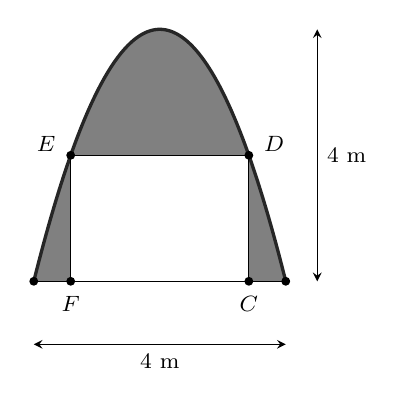
\begin{tikzpicture}[scale=0.8, line join=round, line cap=round, >=stealth, font=\footnotesize]

			% Định nghĩa các tọa độ dựa trên phương trình y = -1/2 x^2 + 8
			\coordinate (A) at (-2, 0);
			\coordinate (B) at (2, 0);
			\coordinate (F) at (-1.414, 0);
			\coordinate (G) at (1.414, 0);
			\coordinate (E) at (-1.414, 2);
			\coordinate (D) at (1.414, 2);
			% Tô màu xám nhạt cho hình chữ nhật MNPQ
			\draw[fill=gray, line width = 1.2pt,draw=none] (-2,0) plot[domain=-2:2] (\x, {-1*\x*\x + 4})--(2,0)--cycle;
			\fill[white] (F) rectangle (D);
			% Vẽ Parabol y = -0.5*x^2 + 8 với tập xác định [-4; 4]
			\draw[line width=1.2pt, black!85] plot[domain=-2:2, samples=100] (\x, {-1*\x*\x + 4});
			% Vẽ đường thẳng đáy AB và khung hình chữ nhật
			\draw (A) -- (B);
			\draw (G) -- (D);
			\draw (D) -- (E);
			\draw (E) -- (F);
			% Vẽ các dấu chấm tròn tại các đỉnh
			\foreach \point in {A, B, D, E,F,G} {
				\fill (\point) circle (2pt);
			}
			\draw[<->] (2.5,0)--(2.5,4)node[right,pos=0.5]{$4$ m};
			\draw[<->] (-2,-1)--(2,-1)node[below,pos=0.5]{$4$ m}; % Đoạn thẳng AB nhãn là a


			% Thêm nhãn tên các điểm
			%\node[below,  yshift=-2pt] at (A) {$A$};
			%\node[below,  yshift=-2pt] at (Q) {$Q$};
			\node[below,  yshift=-2pt] at (G) {$C$};
			\node[below,  yshift=-2pt] at (F) {$F$};

			\node[left,  xshift=-2pt, yshift=4pt] at (E) {$E$};
			\node[right,  xshift=2pt, yshift=4pt] at (D) {$D$};

		\end{tikzpicture}
	}
	\loigiai{
		\begin{center}
			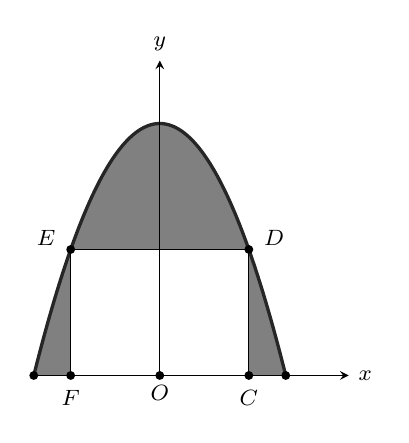
\begin{tikzpicture}[scale=0.8, line join=round, line cap=round, >=stealth, font=\footnotesize]

				% Định nghĩa các tọa độ dựa trên phương trình y = -1/2 x^2 + 8
				\coordinate (A) at (-2, 0);
				\coordinate (B) at (2, 0);
				\coordinate (F) at (-1.414, 0);
				\coordinate (G) at (1.414, 0);
				\coordinate (E) at (-1.414, 2);
				\coordinate (D) at (1.414, 2);
				\coordinate (O) at (0, 0);
				\draw[fill=gray, line width = 1.2pt,draw=none] (-2,0) plot[domain=-2:2] (\x, {-1*\x*\x + 4})--(2,0)--cycle;
				\fill[white] (F) rectangle (D);
				% Vẽ Parabol y = -0.5*x^2 + 8 với tập xác định [-4; 4]
				\draw[line width=1.2pt, black!85] plot[domain=-2:2, samples=100] (\x, {-1*\x*\x + 4});
				% Vẽ đường thẳng đáy AB và khung hình chữ nhật
				\draw (A) -- (B);
				\draw (G) -- (D);
				\draw (D) -- (E);
				\draw (E) -- (F);
				\draw[->](B)--(3,0) node[right]{$x$};
				\draw[->](0,0) node[below ]{$O$}--(0,5) node[above]{$y$};
				% Vẽ các dấu chấm tròn tại các đỉnh
				\foreach \point in {A, B, D, E,F,G,O} {
					\fill (\point) circle (2pt);
				}
				% Thêm nhãn tên các điểm
				%\node[below,  yshift=-2pt] at (A) {$A$};
				%\node[below,  yshift=-2pt] at (Q) {$Q$};
				\node[below,  yshift=-2pt] at (G) {$C$};
				\node[below,  yshift=-2pt] at (F) {$F$};

				\node[left,  xshift=-2pt, yshift=4pt] at (E) {$E$};
				\node[right,  xshift=2pt, yshift=4pt] at (D) {$D$};

			\end{tikzpicture}
		\end{center}
		Chọn hệ trục tọa độ $Oxy$ như hình vẽ trên.\\
		Từ hình vẽ, ta có parabol $(P)$ có dạng là $y=ax^2+bx+c$; $a$,  $b$, $c\in \mathbb{R}$.\\
		Do $(P)$ có đồ thị là parabol có đỉnh $(0;4)$ và đi qua điểm có tọa độ là $(2;0)$ nên
		$$\heva{&b=0\\&c=4\\&4a+2b+c=0}\Leftrightarrow \heva{&a=-1\\&b=0\\&c=4.}$$
		Vậy $(P)$ có phương trình $y=-x^2+4$.\\
		Theo giả thiết điểm $D$ thuộc đồ thị $(P)$ có tung độ bằng $2$ suy ra hoành độ là nghiệm phương trình
		$$-x^2+4=2\Leftrightarrow x=\pm\sqrt{2}.$$
		Theo đồ thị điểm $D$ có hoành độ dương nên $D(\sqrt{2};2)$.\\
		Chiều rộng của cửa là $CF=2\cdot OD=2\sqrt{2}$ m.\\
		Ta có, diện tích của $(P)$ tạo với trục hoành là $S=\displaystyle\int \limits_{-2}^{2}(-x^2+4)\mathrm{\,d}x=\dfrac{32}{3}$ m$^2$.\\
		Diện tích hình chữ nhật $CDEF$ là $S_{CDEF}=2\cdot 2\sqrt{2}=4\sqrt{2}$.\\
		Diện tích cần trang trí là $S_1=S-S_{CDEF}=\dfrac{32}{3}-4\sqrt{2}=\dfrac{32-12\sqrt{2}}{3}$.\\
		Chi phí để trang trí phần tô đậm là $\left(\dfrac{32-12\sqrt{2}}{3}\right)\cdot 1{,}5\approx7{,}5$ (triệu đồng).\\
		Số tiền gia đình đó phải trả để trang trí phần tô đậm là $7{,}5$ (triệu đồng).
	}
\end{ex}

\begin{ex}%[2D1V3-6]
	Trong một bài thực hành huấn luyện quân sự có một tình huống chiến sĩ phải bơi qua sông để tấn công mục tiêu ở ngay phía bờ bên kia sông. Biết rằng lòng sông rộng $100$ m và vận tốc bơi của chiến sĩ bằng một phần ba vận tốc chạy trên bộ. Biết dòng sông là thẳng, mục tiêu cách chiến sỹ $1$ km theo đường chim bay và chiến sỹ cách bờ bên kia $100$ m. Hãy cho biết chiến sỹ phải bơi bao nhiêu mét để đến được mục tiêu nhanh nhất (làm tròn kết quả đến hàng đơn vị)
	\shortans[]{106}
	\loigiai{
		Gọi $A$ là mục tiêu; $B$ là vị trí chiến sỹ và $BD$ là đường bơi của chiến sỹ.\\
		Chọn một đơn vị độ dài là $100$ m suy ra $BC=1$; $AB=10$; $AC=3\sqrt{11}$.\\
		Gọi vận tốc bơi của chiến sỹ là một đơn vị vận tốc thì vận tốc chạy của chiến sỹ là 3 đơn vị vận tốc.\\
		Gọi $x$ là quãng đường chiến sỹ bơi suy ra $BD=x$ ($x>0$).\\
		Vậy quãng đường chiến sỹ chạy là $AD=AC-CD=3\sqrt{11}-\sqrt{x^2-1}$.\\
		Thời gian chiến sỹ đến được mục tiêu là $t=\dfrac{3\sqrt{11}-\sqrt{x^2-1}}{3}+\dfrac{x}{1}=\sqrt{11}-\dfrac{1}{3}\sqrt{x^2-1}+x$.\\
		Xét hàm $f(x)=\sqrt{11}-\dfrac{1}{3}\sqrt{x^2-1}+x$ có $f'(x)=1-\dfrac{1}{3}\dfrac{x}{\sqrt{x^2-1}}=0\Leftrightarrow \hoac{&x=\dfrac{3\sqrt{2}}{4}\text{ (thỏa mãn)}\\&x=-\dfrac{3\sqrt{2}}{4}\text{ (loại)}.}$\\
		Bảng biến thiên
		\begin{center}
			
\begin{tikzpicture}
				\tkzTabInit[lgt=1.2,espcl=3]{$x$ /1, $f'(x)$ /1, $f(x)$ /2}
				{$1$, $\dfrac{3\sqrt{2}}{4}$, $10$}
				\tkzTabLine{,-,0,+,}
				\tkzTabVar{+/ , -/ , +/ }
			\end{tikzpicture}
		\end{center}
		Vậy thời gian chiến sỹ đến mục tiêu ngắn nhất khi $f(x)$ đạt giá trị nhỏ nhất $\Leftrightarrow x=\dfrac{3\sqrt{2}}{4}$.\\
		Vậy chiến sỹ phải bơi $\dfrac{3\sqrt{2}}{4}\cdot 100\approx106$ m.
	}
\end{ex}

\begin{ex}%[2D5V2-3]
	Có hai hộp bóng bàn, các quả bóng bàn có kích thước và hình dạng như nhau. Hộp I chứa $3$ bóng bàn màu trắng và $2$ bóng bàn màu vàng, hộp II chứa $6$ bóng bàn màu trắng và $4$ bóng bàn màu vàng. Lấy ngẫu nhiên $4$ quả bóng bàn ở hộp I bỏ vào hộp II rồi lấy ngẫu nhiên $1$ quả bóng bàn từ hộp II ra. Tính xác suất để quả bóng bàn lấy từ hộp II có màu vàng.
	\shortans[]{0,4}
	\loigiai{
		Gọi $A$: \lq\lq Lấy được quả bóng bàn màu vàng từ hộp II\rq\rq;\\
		$B$: \lq\lq Lấy được $4$ quả bóng bàn ở hộp I, trong đó có đúng 1 quả màu vàng\rq\rq.\\
		Ta có $\overline{B}$: \lq\lq Lấy được 4 quả bóng bàn ở hộp I, trong đó có đúng 2 quả màu vàng\rq\rq.
		\begin{itemize}
			\item \textbf{TH1.} $B$ xảy ra
			\begin{itemize}
				\item Số cách lấy $4$ quả bóng bàn ở hộp I là $\mathrm{C}_5^4$, có $1$ cách lấy 3 quả trắng và $2$ cách lấy $1$ quả vàng.\\
				Ta có $\mathrm{P}\left(B\right)=\dfrac{1\cdot 2}{\mathrm{C}_5^4}=\dfrac{2}{5}$.
				\item Sau khi bỏ $4$ quả ở hộp I sang hộp II thì hộp II sẽ có $9$ quả màu trắng và $5$ quả màu vàng.\\
				Do đó $\mathrm{P}\left(A\mid B\right)=\dfrac{5}{14}$.
			\end{itemize}
		\item \textbf{TH2.} $\overline{B}$ xảy ra
		\begin{itemize}
			\item Số cách lấy $4$ quả ở hộp I là $\mathrm{C}_5^4$, có $\mathrm{C}_3^2$ cách lấy ra $2$ quả trắng và $1$ cách lấy ra $2$ quả màu vàng từ hộp I.\\
			Ta có $\mathrm{P}\left(\overline{B}\right)=\dfrac{\mathrm{C}_3^2\cdot 1}{\mathrm{C}_5^4}=\dfrac{3}{5}$ hoặc có thể tính $\mathrm{P}\left(\overline{B}\right)=1-\mathrm{P}\left(B\right)=1-\dfrac{2}{5}=\dfrac{3}{5}$.
			\item Sau khi bỏ $4$ quả ở hộp I sang hộp II thì hộp II sẽ có $8$ quả màu trắng và $6$ quả màu vàng.
		\end{itemize}
		\end{itemize}
		Vậy $\mathrm{P}\left(A\mid \overline{B}\right)=\dfrac{6}{14}=\dfrac{3}{7}$.\\
		Cuối cùng áp dụng công thức xác suất toàn phần
		$$\mathrm{P}\left(A\right)=\mathrm{P}\left(B\right)\cdot \mathrm{P}\left(A\mid B\right)+\mathrm{P}\left(\overline{B}\right)\cdot \mathrm{P}\left(A\mid \overline{B}\right)=\dfrac{2}{5}\cdot \dfrac{5}{14}+\dfrac{3}{5}\cdot \dfrac{3}{7}=0{,}4.$$
	}
\end{ex}

\Closesolutionfile{ans}
\indapan{4}{ans/De-TB-Yeu-So-6}
